%!TEX program = xelatex
\documentclass[tikz, border=2mm]{standalone}
\usepackage{pgfplots}
\usepackage{xcolor}
\usepgfplotslibrary{colormaps}
\pgfplotsset{compat=1.18}

\begin{document}
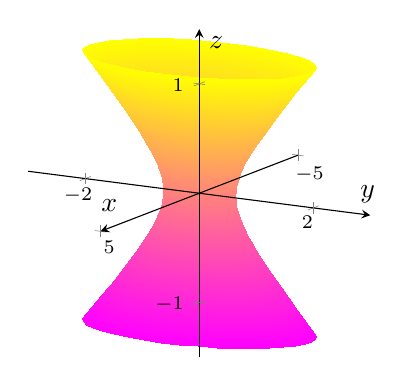
\begin{tikzpicture}
    \begin{axis}[
        view={120}{15},
        axis lines=center,
        xlabel=$x$, ylabel=$y$, zlabel=$z$,
        xmax=5, xmin=-5,       % X轴范围扩展
        ymax=3, ymin=-3,       % Y轴对称范围
        zmax=1.5, zmin=-1.5,   % Z轴对称范围
        tick label style={font=\scriptsize},  % 调大刻度标签
        axis on top,
        colormap/spring
    ]
        \addplot3 [
            surf,
            z buffer=sort,
            samples=40,        % 曲面采样率
            domain=-0.4*pi:0.4*pi, 
            y domain=0:2*pi,
            shader=interp      % 增强着色效果
        ] (
            {0.6*sec(deg(x))*cos(deg(y))},  % 双曲面参数方程
            {0.6*sec(deg(x))*sin(deg(y))},
            {0.4*tan(deg(x))}
        );
    \end{axis}
\end{tikzpicture}
\end{document}